%%%%%%%%%%%%%%%%%%%%%%%%%%%%%%%%%%%%%%%%%
% Jacobs Landscape Poster
% LaTeX Template
% Version 1.0 (29/03/13)
%
% Created by:
% Computational Physics and Biophysics Group, Jacobs University
% https://teamwork.jacobs-university.de:8443/confluence/display/CoPandBiG/LaTeX+Poster
% 
% Further modified by:
% Nathaniel Johnston (nathaniel@njohnston.ca)
%
% This template has been downloaded from:
% http://www.LaTeXTemplates.com
%
% License:
% CC BY-NC-SA 3.0 (http://creativecommons.org/licenses/by-nc-sa/3.0/)
%
%%%%%%%%%%%%%%%%%%%%%%%%%%%%%%%%%%%%%%%%%

%----------------------------------------------------------------------------------------
%	PACKAGES AND OTHER DOCUMENT CONFIGURATIONS
%----------------------------------------------------------------------------------------

\documentclass[final]{beamer}

\usepackage[scale=1.24]{beamerposter} % Use the beamerposter package for laying out the poster
\usepackage{parskip}
\usepackage[justification=centering]{caption}
\usepackage{graphicx, subcaption}
\usetheme{confposter} % Use the confposter theme supplied with this template

\setbeamercolor{block title}{fg=ngreen,bg=white} % Colors of the block titles
\setbeamercolor{block body}{fg=black,bg=white} % Colors of the body of blocks
\setbeamercolor{block alerted title}{fg=white,bg=dblue!70} % Colors of the highlighted block titles
\setbeamercolor{block alerted body}{fg=black,bg=dblue!10} % Colors of the body of highlighted blocks
% Many more colors are available for use in beamerthemeconfposter.sty

%-----------------------------------------------------------
% Define the column widths and overall poster size
% To set effective sepwid, onecolwid and twocolwid values, first choose how many columns you want and how much separation you want between columns
% In this template, the separation width chosen is 0.024 of the paper width and a 4-column layout
% onecolwid should therefore be (1-(# of columns+1)*sepwid)/# of columns e.g. (1-(4+1)*0.024)/4 = 0.22
% Set twocolwid to be (2*onecolwid)+sepwid = 0.464
% Set threecolwid to be (3*onecolwid)+2*sepwid = 0.708

\newlength{\sepwid}
\newlength{\onecolwid}
\newlength{\twocolwid}
\newlength{\threecolwid}
\setlength{\paperwidth}{48in} % A0 width: 46.8in
\setlength{\paperheight}{36in} % A0 height: 33.1in
\setlength{\sepwid}{0.015\paperwidth} % Separation width (white space) between columns
\setlength{\onecolwid}{0.22\paperwidth} % Width of one column
\setlength{\twocolwid}{0.464\paperwidth} % Width of two columns
\setlength{\threecolwid}{0.708\paperwidth} % Width of three columns
\setlength{\topmargin}{-0.5in} % Reduce the top margin size
%-----------------------------------------------------------

\usepackage{graphicx}  % Required for including images
\usepackage{booktabs} % Top and bottom rules for tables


%----------------------------------------------------------------------------------------
%	TITLE SECTION 
%----------------------------------------------------------------------------------------

\title{Data Representations for Unsupervised Learning of RNA Structure} % Poster title

\author{Sitara Persad} % Author(s)
\institute{MIT 6.860/9.520 Project} % Institution(s)

%----------------------------------------------------------------------------------------

\begin{document}

\addtobeamertemplate{block end}{}{\vspace*{2ex}} % White space under blocks
\addtobeamertemplate{block alerted end}{}{\vspace*{2ex}} % White space under highlighted (alert) blocks

\setlength{\belowcaptionskip}{2ex} % White space under figures
\setlength\belowdisplayshortskip{2ex} % White space under equations

\begin{frame}[t] % The whole poster is enclosed in one beamer frame

\begin{columns}[t] % The whole poster consists of three major columns, the second of which is split into two columns twice - the [t] option aligns each column's content to the top

\begin{column}{\sepwid}\end{column} % Empty spacer column

\begin{column}{\onecolwid} % The first column

%----------------------------------------------------------------------------------------
%	OBJECTIVES
%----------------------------------------------------------------------------------------

\begin{alertblock}{Introduction}
Beyond carrying genetic information, RNA folds into higher order structures that carry out key cell process. RNA structure prediction algorithms do not reflect the chemical environment of the cell, which affects accuracy. Experimental data constrain these predictions, but compute only average signal over all RNA molecules, obscuring the structures which perform different functions.

We  study low dimensional data representation via distance preservation and minimal reconstruction error to identify and cluster individual structures. We implement t-SNE, multi-dimensional scaling (MDS), autoencoders and deep embedded clustering and evaluate their performance on a test molecule. 
\end{alertblock}

%----------------------------------------------------------------------------------------
%	INTRODUCTION
%----------------------------------------------------------------------------------------

\begin{block}{RNA Structure Probing}
Dimethyl Sulfate probes RNA structure \textit{in vivo} by modifying the Watson-Crick position of A and C bases. 
TGIRT enzyme converts modifications to mutations that are sequenced in the DNA. \cite{zubradt2017dms}.

\begin{figure}[!ht]
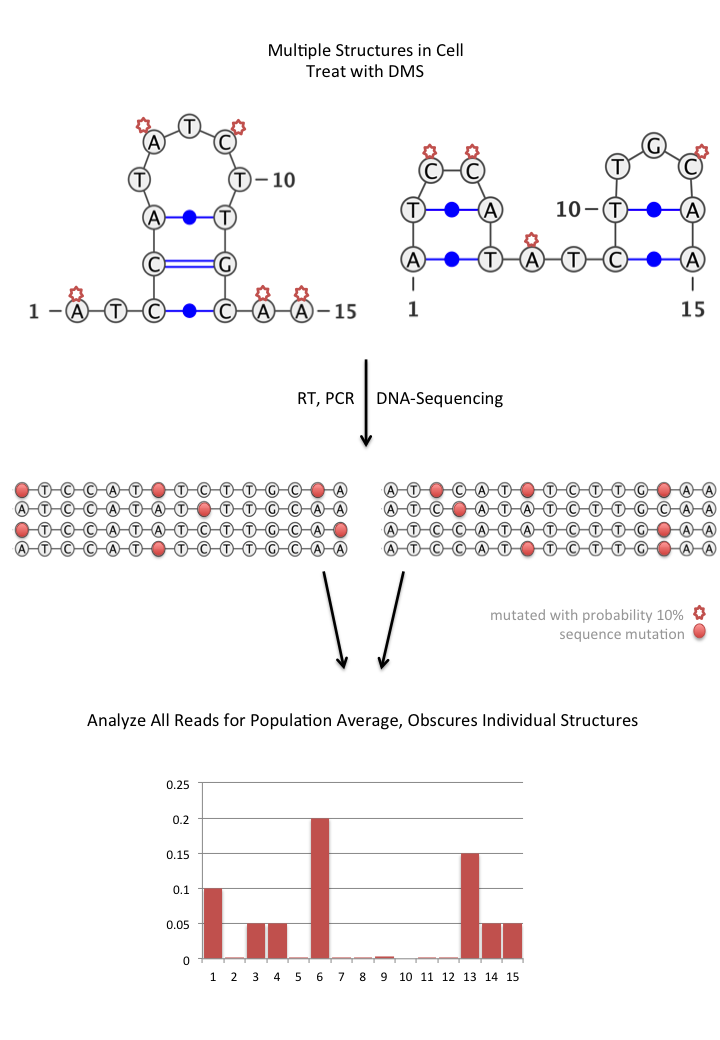
\includegraphics[width=0.9\linewidth]{images/dms_process.png}
\caption{Experimental Assay for Determining RNA Structure Constraints}
\end{figure}

\end{block}


%------------------------------------------------

%----------------------------------------------------------------------------------------

\end{column} % End of the first column

\begin{column}{\sepwid}\end{column} % Empty spacer column

\begin{column}{\onecolwid} % The first column

\begin{block}{Method}

\begin{enumerate}
\item Synthesize two structural forms of a small RNA molecule which differ at a single genetic locus as a \textbf{test molecule} (structure membership typically unknown).

\begin{figure}[!ht]
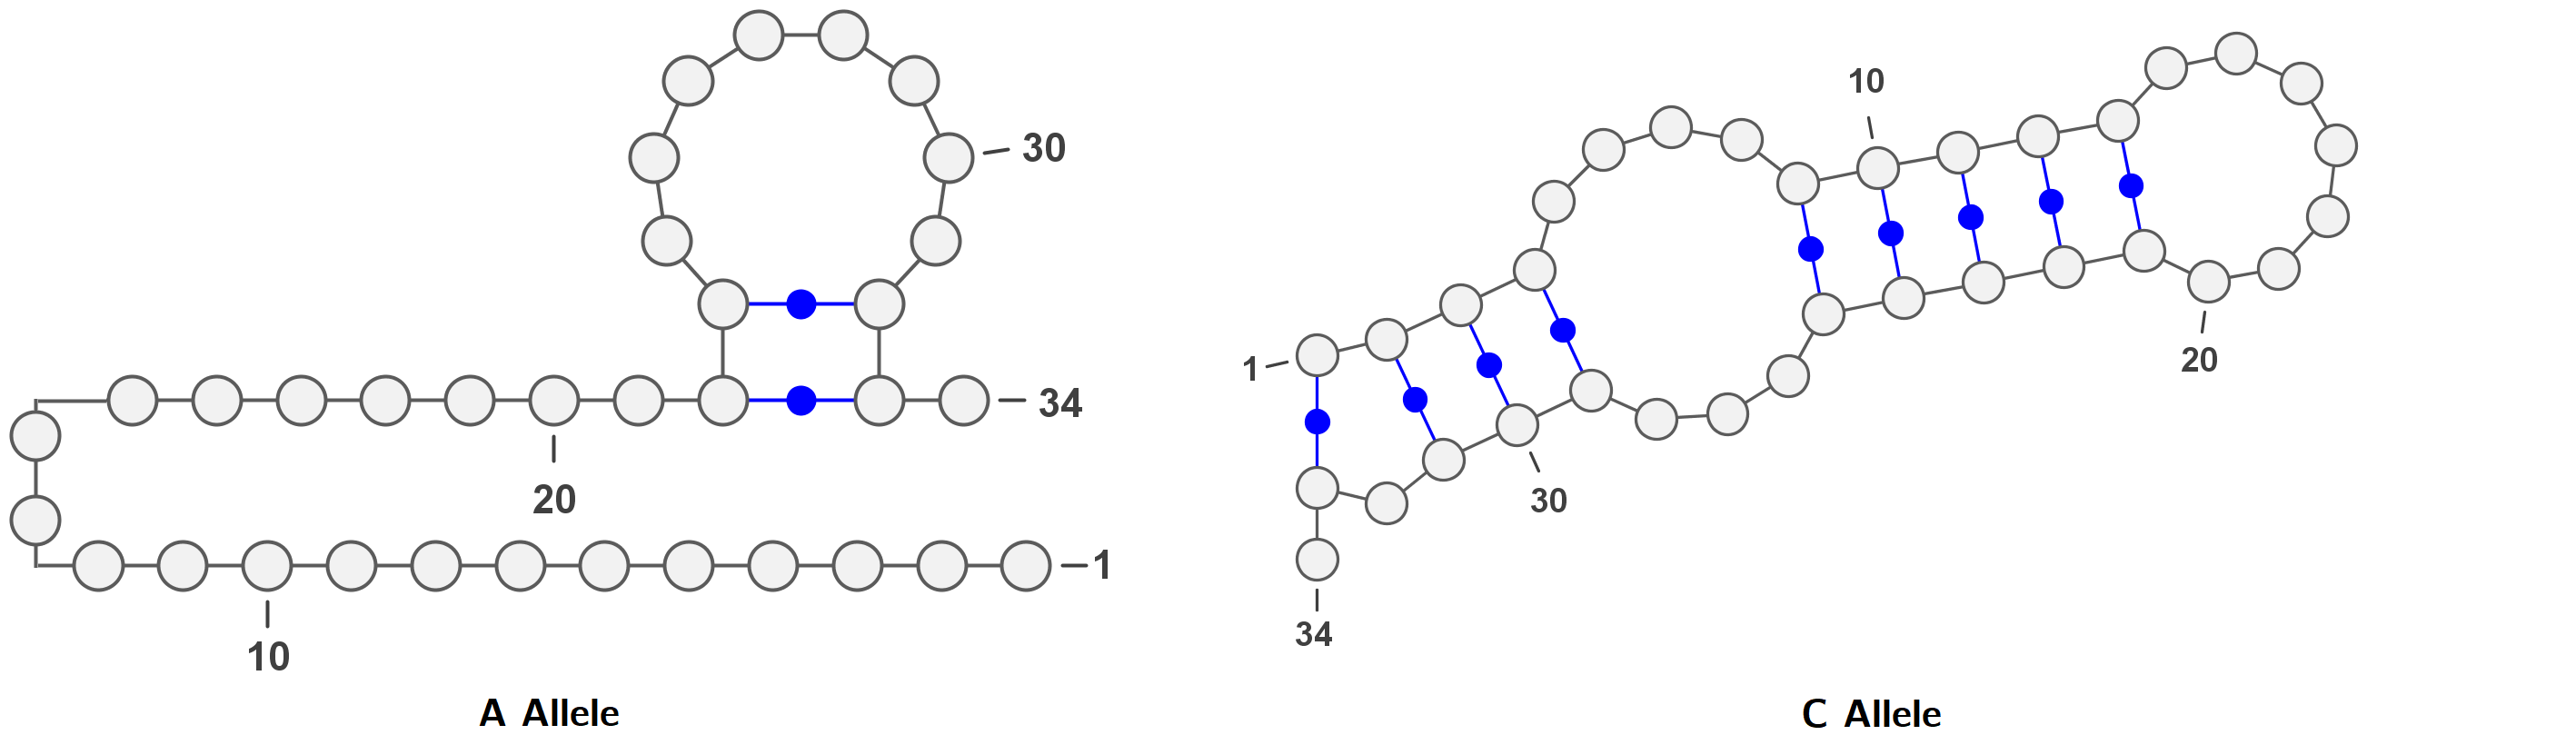
\includegraphics[width=0.9\linewidth]{images/alleles.png}
\caption{Multiple Structures Mixed at Ratio 1:3 and Probed In Vitro}
\end{figure}

\item Identify \textbf{unique reads}.
\item Learn lower-dimensional representation of reads for clustering, using distance preservation methods and reconstruction algorithms. 
\end{enumerate}
\end{block}

\begin{block}{Autoencoder}

\begin{figure}[!ht]
\begin{subfigure}{.5\textwidth}
    \centering
    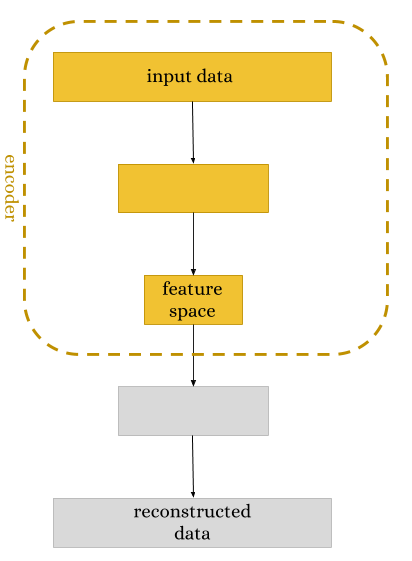
\includegraphics[width=.8\linewidth]{images/encoder-decoder.png}
    \caption{Autoencoder Architecture}
\end{subfigure}%
\begin{subfigure}{.5\textwidth}
    \centering
    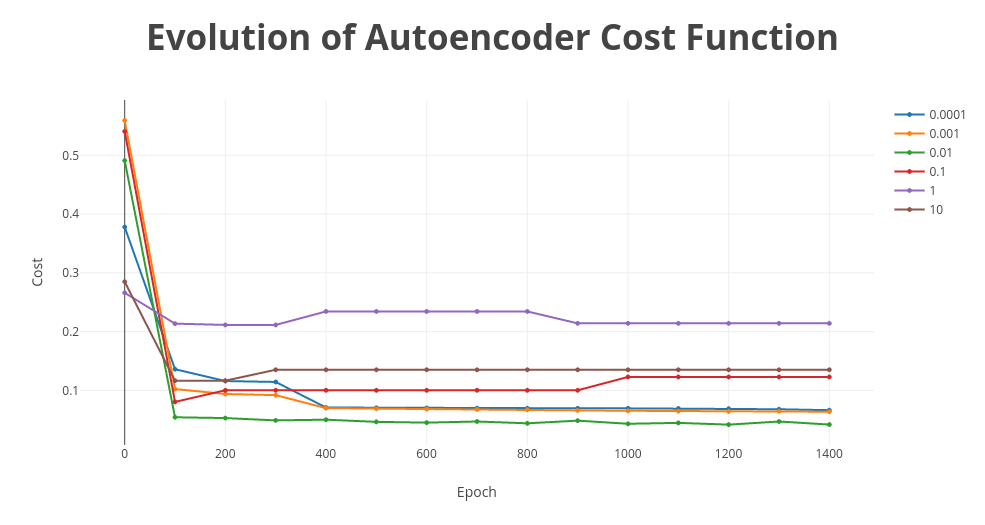
\includegraphics[width=.9\linewidth]{images/ae_cost.png}
    \caption{Autoencoder converges to minimal reconstruction cost}
\end{subfigure}
\end{figure}
   
\begin{figure}[!ht]
    \centering
    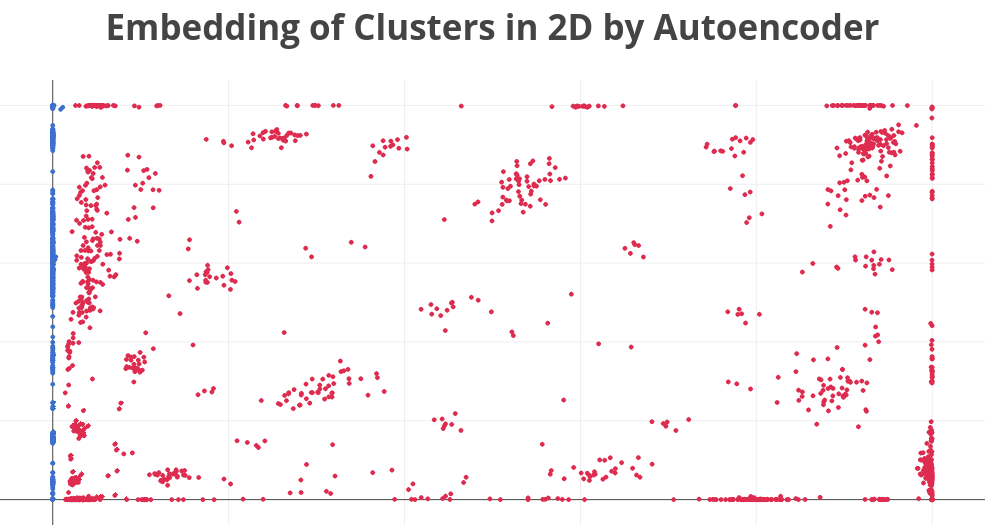
\includegraphics[width=.9\linewidth]{images/ae_embed.png}
    \caption{Autoencoder perfectly separates data but obscures number of true clusters}
\end{figure}

\begin{figure}[!ht]
    \centering
    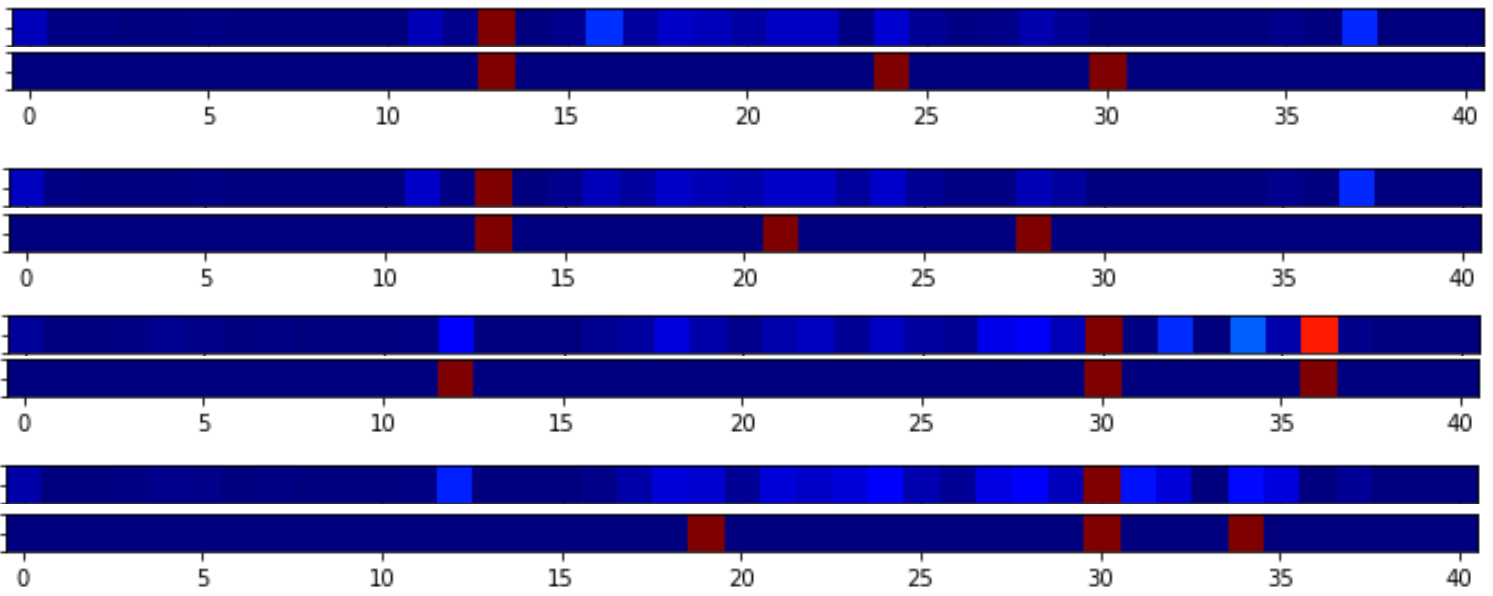
\includegraphics[width=.9\linewidth]{images/reconstruct.PNG}
    \caption{Sample reconstruction (above) from original (below)}
\end{figure}
\end{block}

%------------------------------------------------

%----------------------------------------------------------------------------------------

\end{column} % End of the first column


\begin{column}{\sepwid}\end{column} % Empty spacer column

\begin{column}{\onecolwid} % The third column

%----------------------------------------------------------------------------------------
%	CONCLUSION
%----------------------------------------------------------------------------------------

\begin{block}{Distance Preservation}

$D$ is the matrix of Hamming distances between reads.

\begin{enumerate}
\item t-SNE \cite{maaten2008visualizing} minimizes divergence between distribution of embedded points, $y$, and distribution defined original dissimilarity matrix. 

\item MDS \cite{kruskal1964nonmetric} minimizes the difference between the distance between points in the embedded space and original dissimilarity matrix. 
\begin{figure}[!ht]
\begin{subfigure}{.5\textwidth}
    \centering
    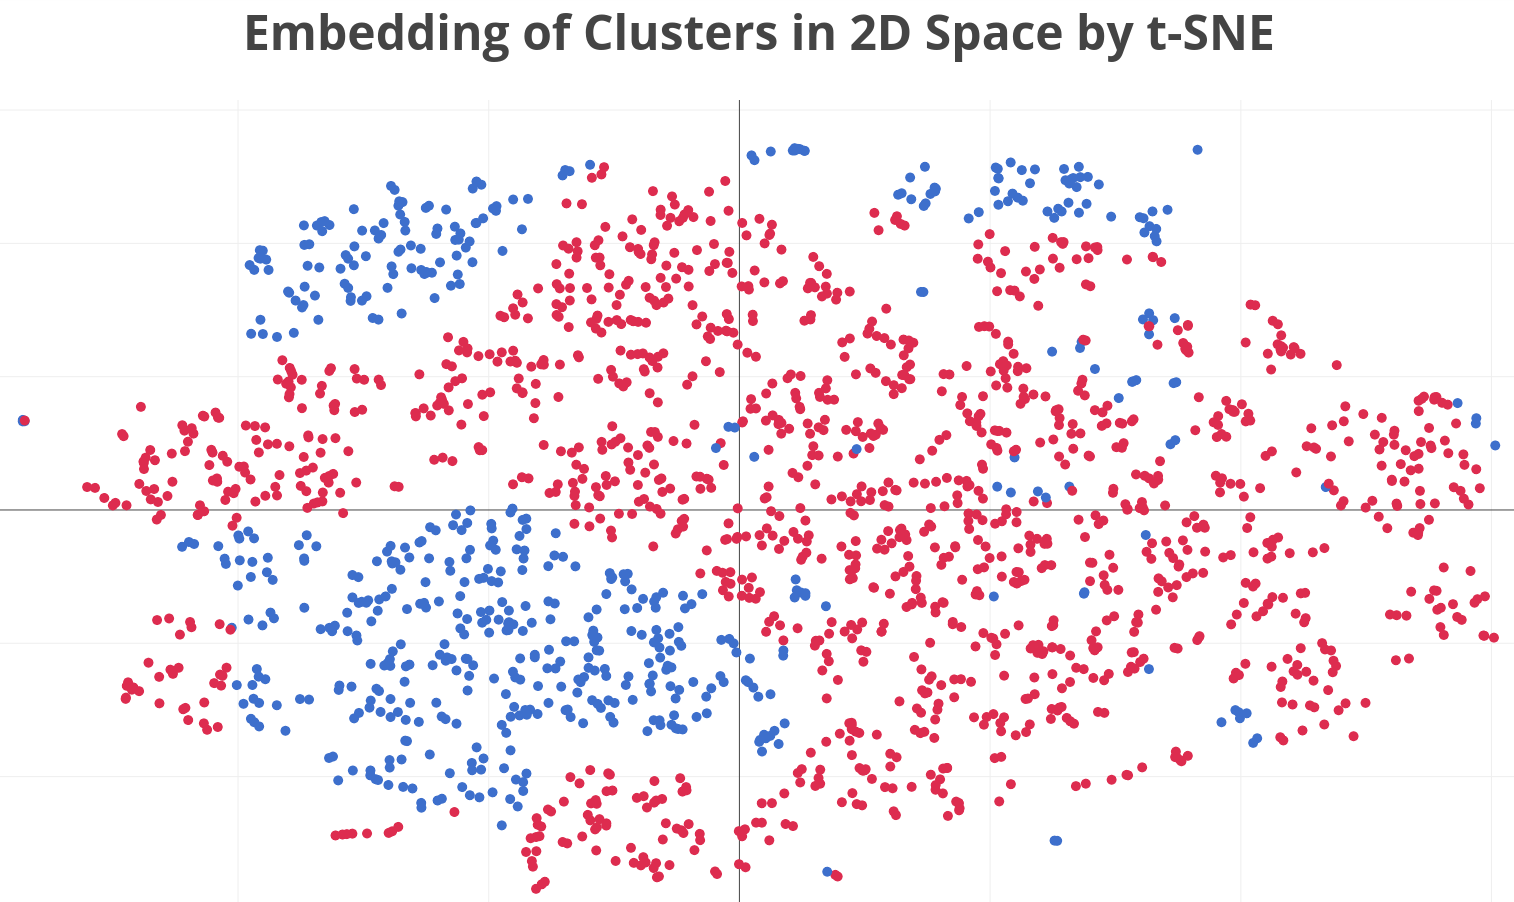
\includegraphics[width=.9\linewidth]{images/tSNE_noNN.png}
    \caption{tSNE Fails to Separate Clusters in 2D}
\end{subfigure}%
\begin{subfigure}{.5\textwidth}
    \centering
    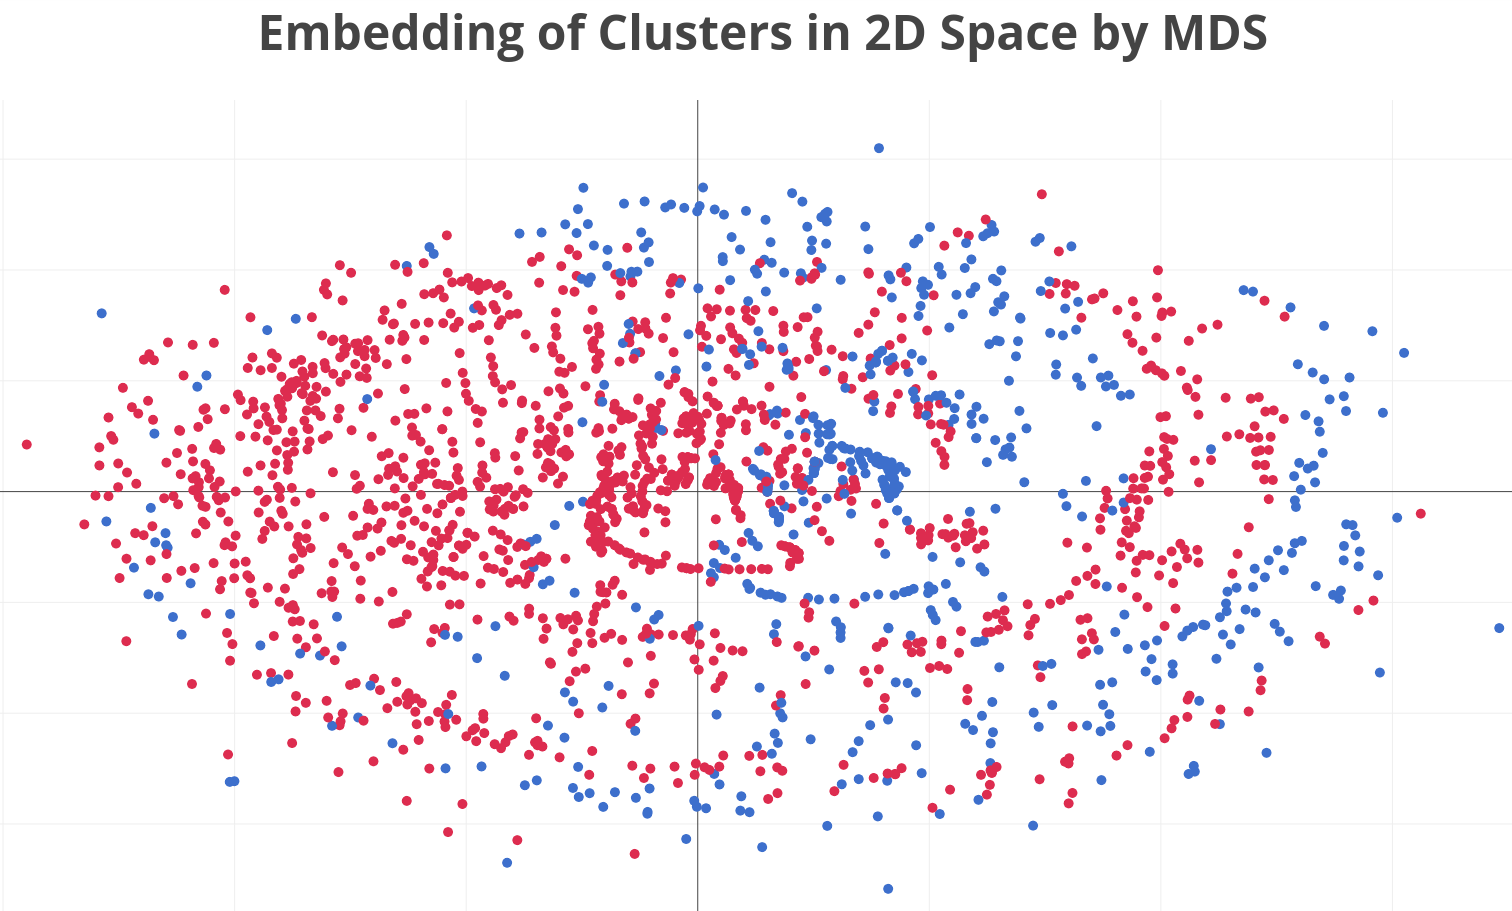
\includegraphics[width=.9\linewidth]{images/MDS_noNN.png}
    \caption{MDS Fails to Separate Clusters in 2D}
\end{subfigure}
\end{figure}

\end{enumerate}
\end{block}

\begin{block}{Distance Preservation + kNN}

We propose a hybrid method combining k-nearest neighbors.

\begin{figure}[!ht]
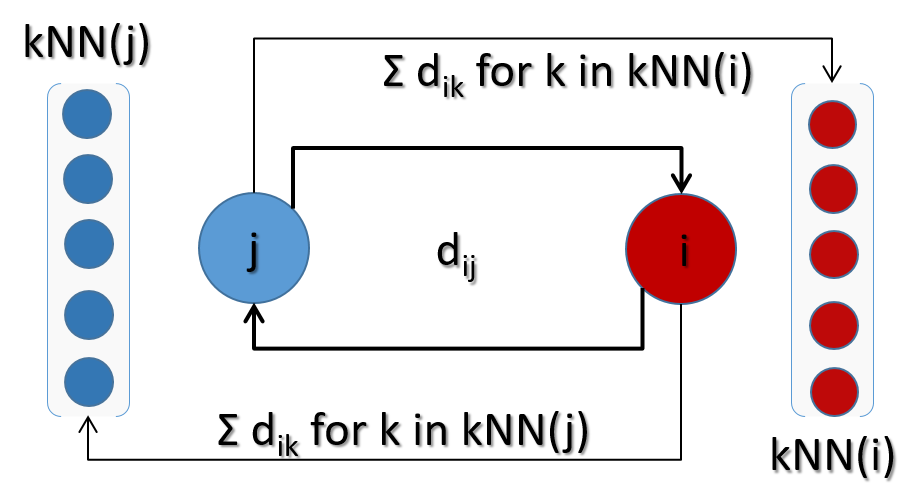
\includegraphics[width=0.4\linewidth]{images/kNN_dist.PNG}
\caption{Include average distance from $x_i$ to kNN of $x_j$}
\end{figure}

\begin{align*}
\delta_{ij} = D_{ij} + \alpha (\Sigma_{k \in KNN(j)} D_{ik} + \Sigma_{k \in KNN(i)} D_{jk}) 
\end{align*}
\vspace{10mm}

\begin{figure}[!ht]
\begin{subfigure}{.5\textwidth}
    \centering
    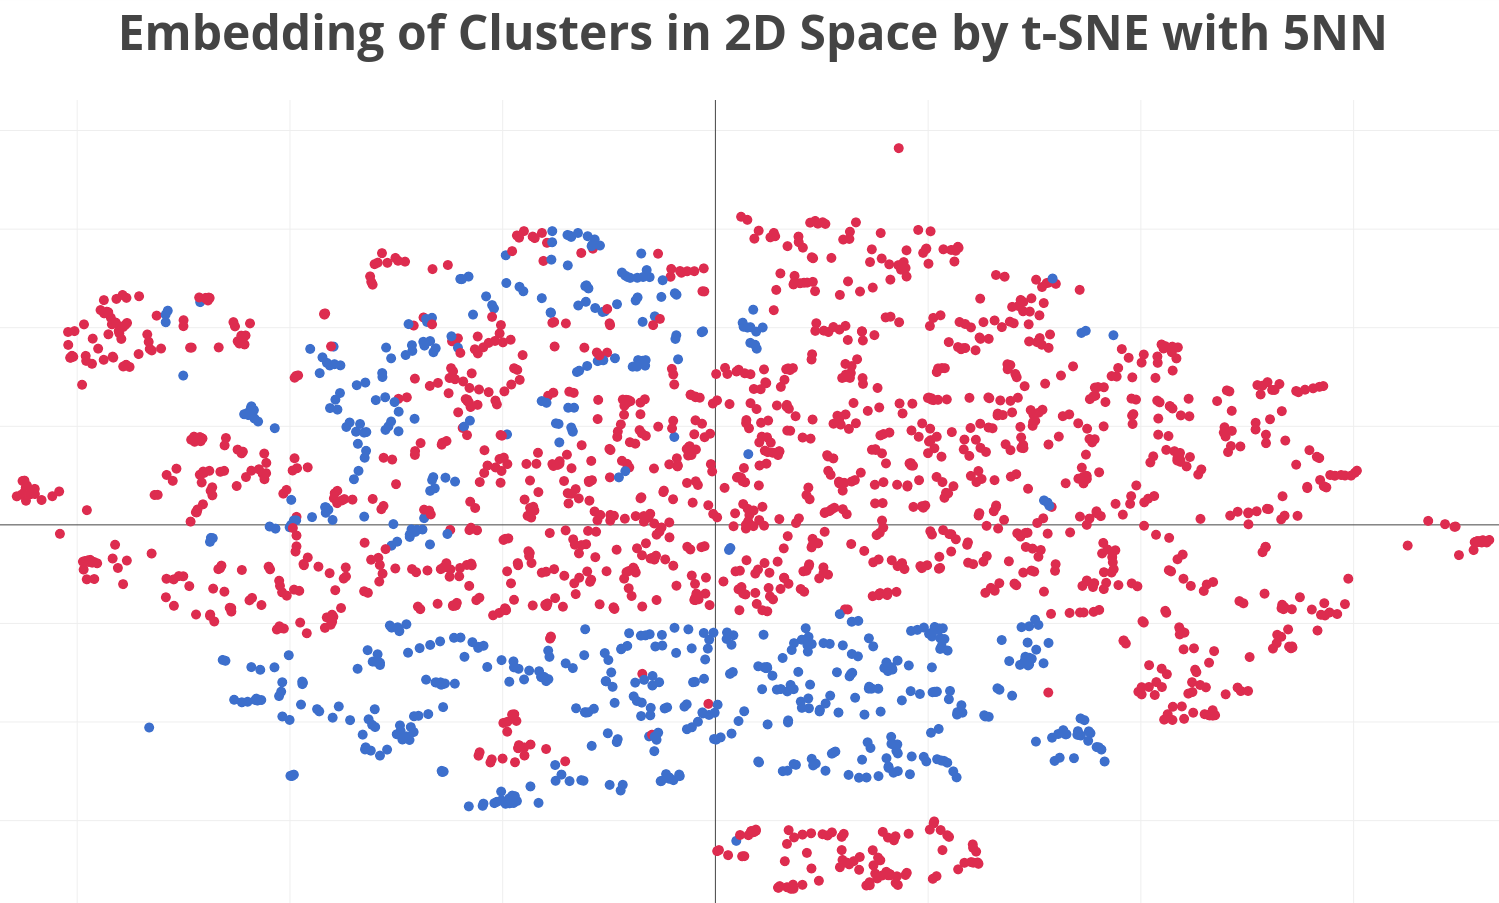
\includegraphics[width=.9\linewidth]{images/tSNE_5NN.png}
    \caption{tSNE with 5NN Fails to Separate Clusters in 2D}
\end{subfigure}%
\begin{subfigure}{.5\textwidth}
    \centering
    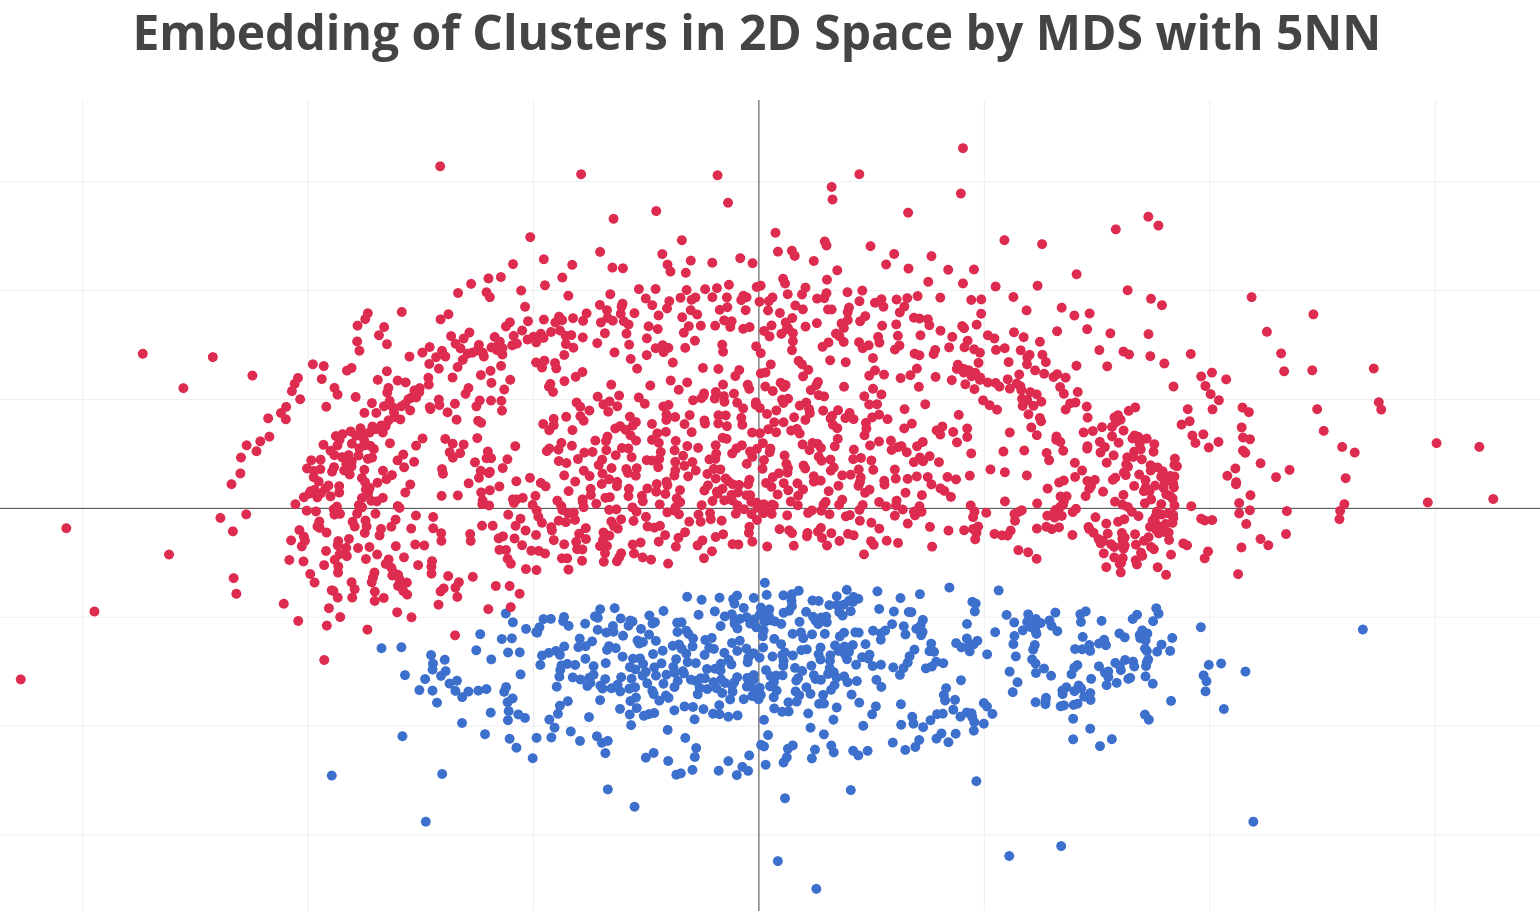
\includegraphics[width=.8\linewidth]{images/MDS_5NN.png}
    \caption{MDS with 5NN Separates Clusters Well in 2D}
\end{subfigure}
\end{figure}

\vspace{10mm}
\begin{figure}[!ht]
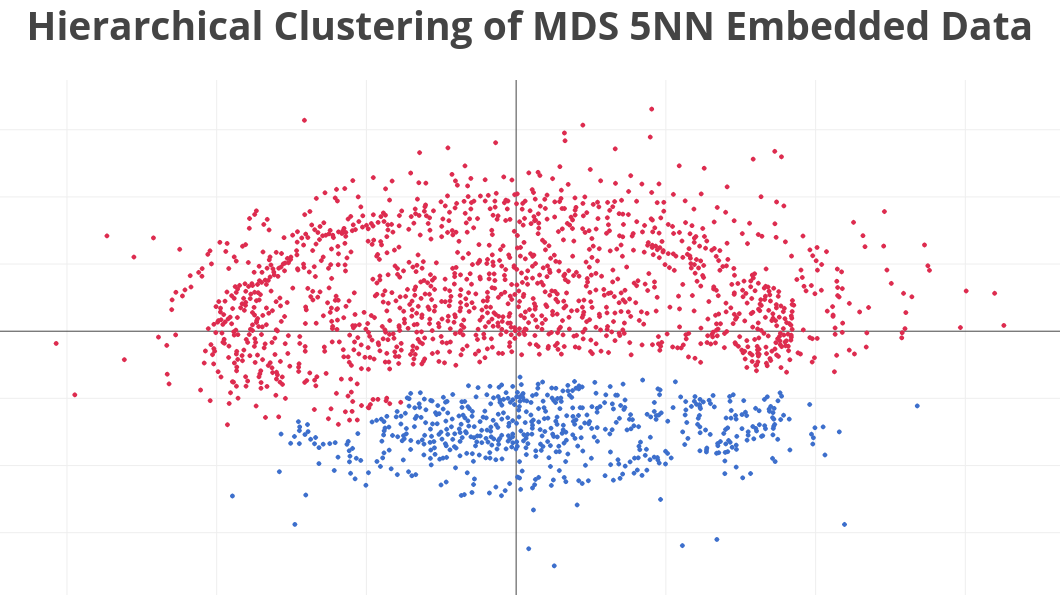
\includegraphics[width=0.9\linewidth]{images/AG_cluster.png}
\caption{Hierarchical Clustering Recovers Structures with 98.5\% Accuracy}
\end{figure}

\end{block}




%----------------------------------------------------------------------------------------

\end{column} % End of the third column

\begin{column}{\sepwid}\end{column} % Empty spacer column

\begin{column}{\onecolwid} % The fourth column

%----------------------------------------------------------------------------------------
%	CONCLUSION
%----------------------------------------------------------------------------------------
\begin{block}{Deep Embedded Clustering }

\begin{figure}[!ht]
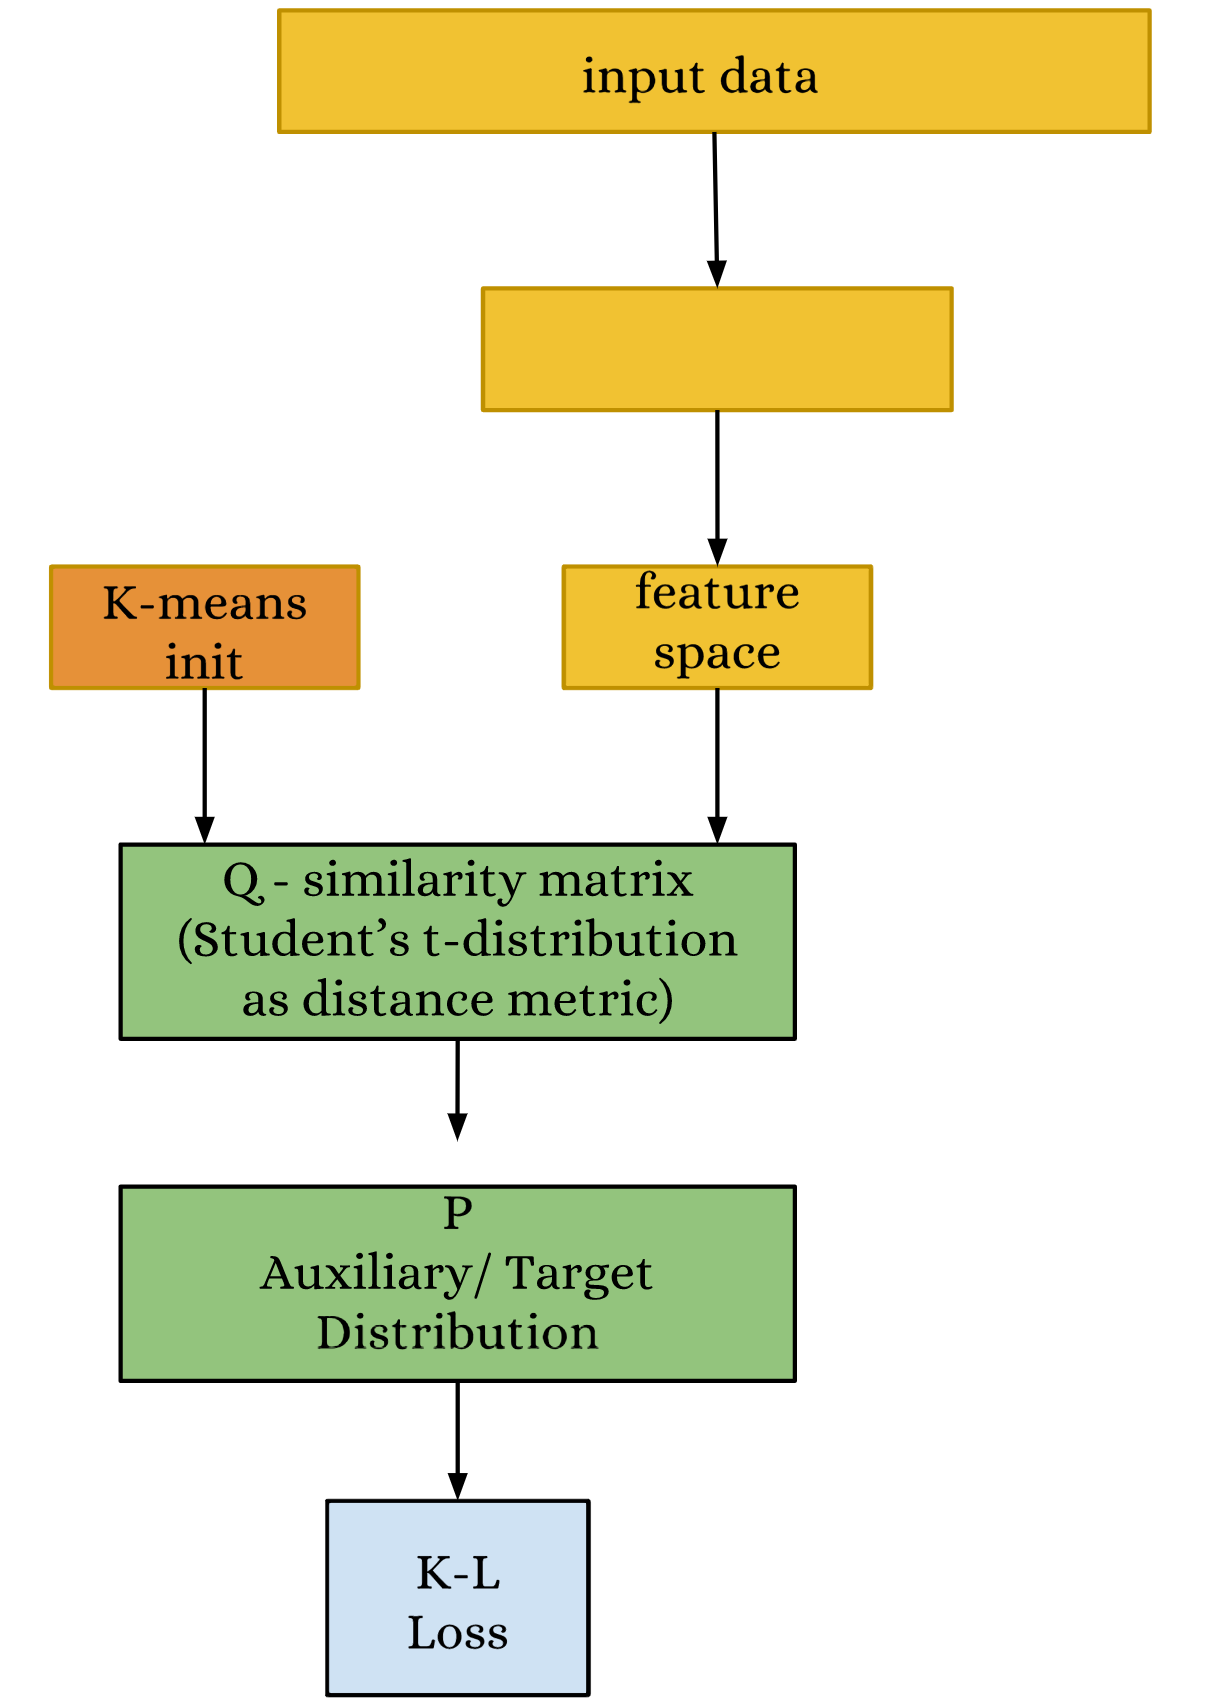
\includegraphics[angle=-90, width=0.5\linewidth]{images/architecture.png}
\caption{DEC uses autoencoder + distance preservation from a cluster exemplar to simultaneously learn encoding and assignments}
\end{figure}

\begin{figure}[!ht]
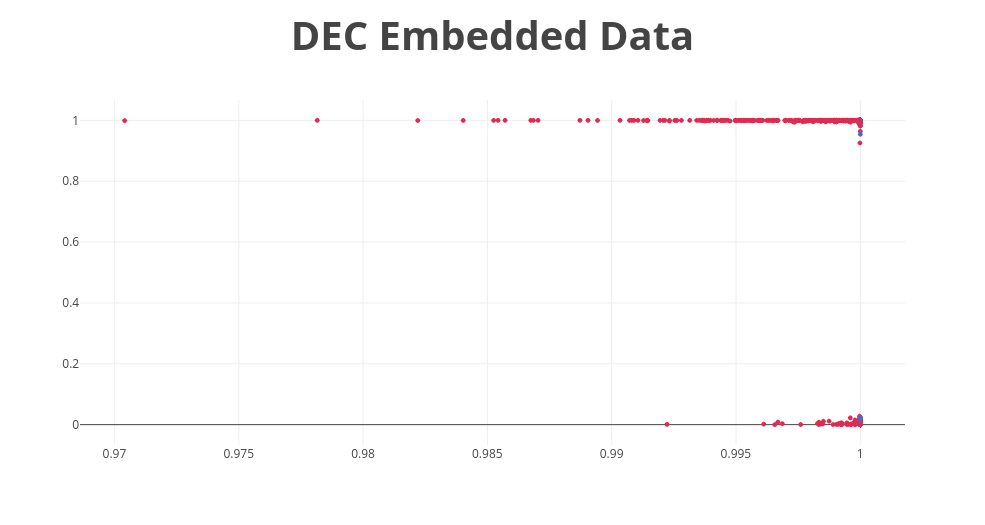
\includegraphics[width=0.8\linewidth]{images/DEC_embed.png}
\caption{DEC fails to separate data, achieving 66.3\% accuracy.}
\end{figure}

\end{block}

\begin{block}{Conclusion}
t-SNE and MDS cannot separate the sparse sequence reads. However, if we include nearest neighbours, we can visualize the number of structures using MDS and perform clustering.

Autoencoders separate the data in 2D, but do not allow us to infer the number of structures present. Deep Embedded Clustering does not separate the data, and fails to produce accurate clustering.

Next steps are to benchmark longer molecules, molecules with increased similarity, and structures mixed in smaller ratios
\end{block}


%----------------------------------------------------------------------------------------
%	REFERENCES
%----------------------------------------------------------------------------------------

\begin{block}{References}

\nocite{*} % Insert publications even if they are not cited in the poster
\small{\bibliographystyle{unsrt}
\bibliography{sample}\vspace{0.75in}}

All code and data available upon request.
\end{block}

%----------------------------------------------------------------------------------------

\end{column} % End of the fourth column

\end{columns} % End of all the columns in the poster

\end{frame} % End of the enclosing frame

\end{document}
